\documentclass[12pt,a4paper]{report}

\usepackage[english]{babel}
\usepackage[utf8]{inputenc}

\usepackage{amsmath}
\usepackage{amsfonts}
\usepackage{amssymb}

\usepackage{graphicx}

\usepackage{ragged2e}

\usepackage{float}
\usepackage{booktabs}
\usepackage{multirow}
\usepackage{appendix}
\usepackage{listings}

%\usepackage{minted}

\usepackage[left=2cm,right=2cm,top=2cm,bottom=2cm]{geometry}

%\usepackage[square,numbers]{natbib}

%\usepackage[
%backend=biber,
%style=alphabetic,
%sorting=ynt
%]{biblatex}
%\addbibresource{bibliography.bib}

\author{Fahim Masud Choudhury}
\title{Performance Analysis of HWMP, AODV and OLSR Protocol in Wireless Mesh Networks and Improvement of OLSR using NS-3}
% arara: indent

\begin{document}
\maketitle
\tableofcontents
\listoffigures

\newpage
\begin{center}
\section*{Acknowledgment}
\justify
First and foremost, I would like to thank God Almighty for giving me the strength to finish this work. The satisfaction that accompanies the successful completion of this thesis would be incomplete without the mention of people whose ceaseless cooperation made it possible, whose constant guidance and encouragement crown all efforts with success. I am grateful to my honorable project Supervisor Mir Md. Saki Kowsar, Assistant Professor, Department of Computer Science and Engineering, Chittagong University of Engineering and Technology, for the guidance, inspiration and constructive suggestions which were helpful in the preparation of this project. I also convey special thanks and gratitude to Professor Dr. Kaushik Deb, honorable head of the Department of Computer Science and Engineering for his kind advice. I would also like to extend my gratitude to all of my teachers for their valuable guidance in every step of mine during the four years of learning stage. Finally I would like to thank my friends, senior, juniors and the staffs of the department for their valuable suggestion and assistance that has helped in successful completion of the project.
\end{center}


\newpage
\begin{center}
\section*{Abstract}
\justify
Wireless Mesh Networks (WMNs) are a radio-based network technology that has gained considerable importance in network research community. It is a multi-hop wireless access network where nodes can act both as a host as well as a router. One of the factors that influence the performance of WMNs is the underlying routing protocol used. Since implementation of wireless routing protocols in a real test bed is difficult, hence, simulation environment is being considered for performance evaluation of a routing protocol in a wireless scenario. Recently, a new network simulator called NS-3, which is in its developing stage, demands a great potential (as claimed by the developers group) for performance analysis of different routing protocols. In this project we aim to implement and analyze the performance of Hybrid Wireless Mesh Protocol (HWMP), Optimized Link State Routing Protocol (OLSR) and Ad hoc On-Demand Distance Vector (AODV) routing protocol in Network Simulator 3 (ns-3). An improved OLSR protocol is also proposed and its performance has been measured. Finally, extensive simulations have been carried out for calculation of Throughput, Packet Delivery Fraction (PDF) and End-to-end delay.

\end{center}

\chapter{Introduction}
\section{Motivation of the Work}
Wireless mesh networks have recently gained a lot of popularity due to their rapid deployment and instant communication capabilities. These networks comprise of somewhat static multi-radio Mesh Routers, which essentially provide connectivity between the mobile single-radio mesh clients. Special routing protocols are employed, which facilitate routing between the mesh routers as well as between the mesh routers and the mobile clients. The routing (or path selection) protocol is used to discover and maintain multi-hop paths in the mesh network. There have been much work going on in routing protocols. At present, almost 70 routing protocols have been proposed for WMNs. But few of these have supports in ns-3. So, the performance analysis of these ns-3 supported routing protocols is essential to simulate the network. Besides, OLSR  protocol is a widely used routing protocols for MANETs and WMNs. It is also implemented in ns-3. So the performance analysis of OLSR and improving this protocol is also a demanding task.

\section{Contribution of the Work}
The objective of this project is to evaluate the performance of wireless mesh networks
using AODV, DSDV and OLSR protocols in terms of different parameters. 
An improved OLSR protocol is also proposed and it's performance has been analyzed. Finally, different graphs are generated to evaluate the performance with specified parameters.

\section{Organization of the Project}
The remainder of the report is organized as follows. In the next chapter, an overview of our project related terminologies are explained and contains brief discussion on previous works that is already implemented with their limitations. Chapter 3 describes the working procedure of our proposed system. In Chapter 4, we have illustrated our implementation of the project in details. Chapter 5 focuses on the experimental result of the proposed system. The thesis concludes with a summary of research contributions and future plan of our work in chapter 6. This thesis contains an appendix intended for persons who wish to explore the source code. 


\chapter{Literature Review}

\section{Wireless Mesh Network}
As various wireless networks evolve into the next generation to provide better services, a key technology, wireless mesh networks (WMNs) has emerged recently. In WMNs, nodes are comprised of mesh routers and mesh clients. Each node operates not only as a host but
also as a router, forwarding packets on behalf of other nodes that may not be within direct
wireless transmission range of their destinations. A WMN is dynamically self-organized and self-configured, with the nodes in the network automatically establishing and maintaining
mesh connectivity among themselves.
Conventional nodes, e.g., desktops, laptops, PDAs, PocketPCs, phones, equipped with
wireless network interface cards (NICs) can be connected directly to wireless mesh routers.
Customers without wireless NICs can access WMNs by connecting to wireless mesh
routers through, for example, Ethernet. Thus, WMNs will greatly help users to be always-
on-line anywhere anytime. Moreover, the gateway/bridge functionalities in mesh routers
enable the integration of WMNs with various existing wireless networks such as cellular
systems, wireless sensor networks, wireless-fidelity (Wi-Fi) systems and worldwide
inter-operability for microwave access (WiMAX)networks.


\subsection{Network Architecture}
WMNs consist of two types of nodes: mesh routers and mesh clients. Other than the routing
capability for gateway/repeater functions as in a conventional wireless router, a wireless mesh
router contains additional routing functions to support mesh networking. To further improve
the flexibility of mesh networking, a mesh router is usually equipped with multiple wireless
interfaces built on either the same or different wireless access technologies.

Mesh clients also have the necessary functions for mesh networking, and thus can also
work as a router in WMN. However, gateway or bridge functions do not exist in these nodes.
In addition, mesh clients usually have only one wireless interface. As a consequence, the
hardware platform and the software for mesh clients can be much simpler than those for mesh
routers. Mesh clients have a greater variety of devices compared to mesh routers. They can be
a laptop/desktop PC, pocket PC, PDA, IP phone, RFID reader, BACnet (Building Automation
and Control network) controller, and many other devices

The architecture of WMNs can be classified into three main groups based on the
functionality of the nodes.

\subsubsection{Infrastructure/Backbone WMNs}
Infrastructure/Backbone WMN includes mesh routers that form
an infrastructure for clients that connect to them. The WMN infrastructure/backbone can be built using various types of radio technology, in addition to the heavily used
IEEE 802.11 technology. The mesh routers form a mesh of self-configuring, self-
healing links among themselves. With gateway functionality, mesh routers can be
connected to the Internet. This approach, also referred to as infrastructure meshing,
provides backbone for conventional clients and enables the integration of WMNs
with existing wireless networks, through gateway/bridge functionalities in mesh
routers.
\begin{figure}[hbtp]
\centering
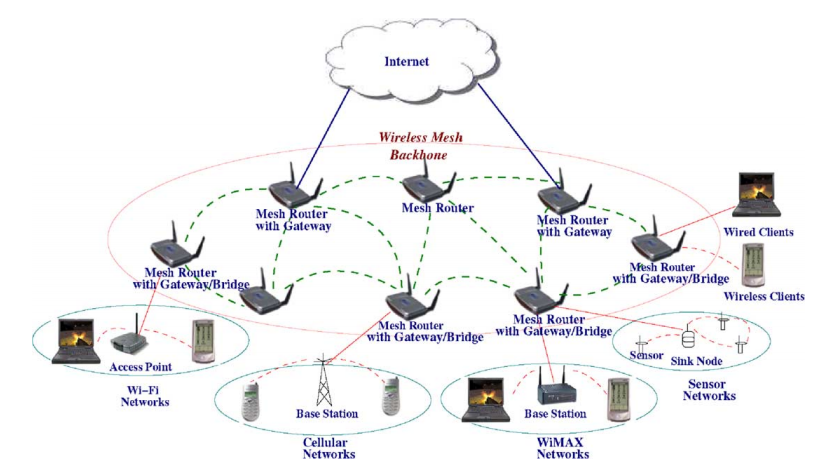
\includegraphics[scale=0.75]{infrastructure-mesh-clear.png}
\caption{Infrastructure/Backbone WMN}
\end{figure}

Infrastructure/Backbone WMNs are the most commonly used type. For example,
community and neighborhood networks can be built using infrastructure meshing.
The mesh routers are placed on the roofs of houses in a neighborhood, and these
can serve as access points for users in homes and along the roads. Typically, two
types of radio are used in the routers, i.e., for backbone communication and for user
communication. The mesh backbone communication can be established using long-
range communication techniques including, for example, directional antennas.

\subsubsection{Client WMNs}
Client meshing provides peer-to-peer networks among client devices.
In this type of architecture, client nodes constitute the actual network to perform
routing and configuration functionalities as well as providing end-user applications to
customers. Hence, a mesh router is not required for this type of network.
\begin{figure}[hbtp]
\centering
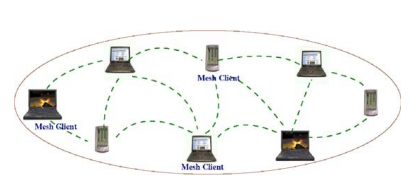
\includegraphics[scale=.5]{client-wmn.png}
\caption{Client WMNs}
\end{figure}


\subsubsection{Hybrid WMNs}
This architecture is the combination of infrastructure and client
meshing. Mesh clients can access the network through mesh
routers as well as directly meshing with other mesh clients. While the infrastructure
provides connectivity to other networks such as the Internet, Wi-Fi, WiMAX, cellular,
and sensor networks, the routing capabilities of clients provide improved connectivity
and coverage inside the WMN.
\begin{figure}[hbtp]
\centering
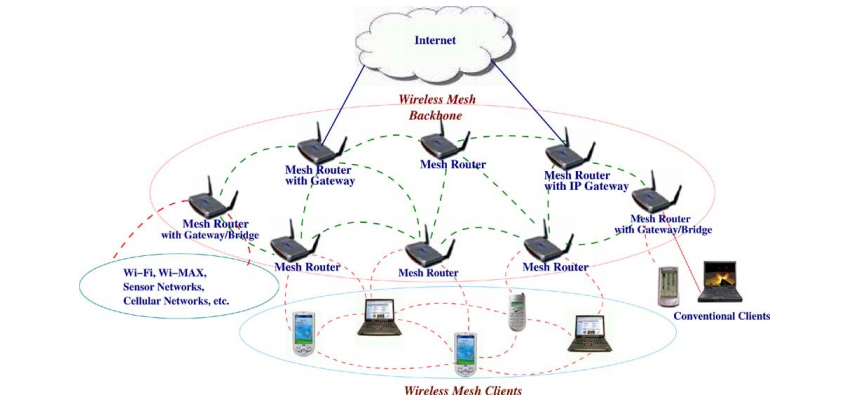
\includegraphics[scale=0.5]{hybrid-wmn.png}
\caption{Hybrid WMNs}
\end{figure}


%\subsection{Management}
%\subsection{Operation}

\subsection{Application}
Research and development of WMNs is motivated by several applications which clearly
demonstrate the promising market, but, at the same time, these applications cannot be
supported directly by other wireless networks such as cellular systems, ad hoc networks,
wireless sensor networks, standard IEEE 802.11, etc. In this section, we discuss these
applications.
\begin{itemize}
\item Broadband home networking
\item Community and neighborhood networking
\item Enterprise networking
\item Metropolitan area networks (MAN)
\item Transportation systems
\item Building automation
\item Health and medical systems
\item Security surveillance systems
\end{itemize}
In addition to the above applications, WMNs can also be applied to spontaneous
(emergency/disaster) networking and P2P communications. For example, wireless networks
for an emergency response team and firefighters do not have in-advance knowledge of
where the network should be deployed. By simply placing wireless mesh routers in
desired locations, a WMN can be quickly established.
For a group of people holding
devices with wireless networking capability, e.g., laptops and PDAs, P2P communication
anytime anywhere is an efficient solution for information sharing. WMNs are able to meet this demand. These applications illustrate that WMNs are a superset of ad hoc networks, and
thus, can accomplish all functions provided by ad hoc networking.

\section{Routing Protocols}
A routing protocol for WMNs can be proactive or reactive. For proactive routing, a routing
path between two nodes is established before any traffic flow is initiated between them. A
reactive routing starts to set up a routing path for two nodes only after traffic is generated
between these two nodes.
A routing protocol can be static or dynamic depending whether or not the network
experiences variations in topology, link quality, traffic load, and so on. In a wired network,
there exist many scenarios where static routing can find many applications. For a multihop
wireless network like a WMN, routing usually needs to be dynamic owing to node mobility,
link instability, topology change, traffic variations, etc. Two popular dynamic routing
schemes are distance vector routing and link state routing, which were proposed for
wired networks and have become the cornerstone of many dynamic routing protocols of
MANETs and WMNs.

\subsection{Reactive Protocols}
Reactive protocols seek to set up routes on-demand. If a node wants to initiate communication with a node to which it has no route, the routing protocol will try to establish such a route.
Reactive protocol searches for the route in an on-demand 
manner and set the link in order to send out and accept the 
packet from a source node to destination node. Route 
discovery process is used in on demand routing by flooding 
the route request (RREQ) packets throughout the network.
Examples of reactive routing protocols are the dynamic 
source Routing (DSR), ad hoc on-demand distance vector 
routing (AODV).


\subsection{Proactive Protocols}
Table-driven or proactive routing protocols establish routes in advance, i.e., these
protocols assume that it is more efficient to determine routes regularly; as soon as a
node tries to send data packets, the reasonable assumption (hope) is that the route
needed has already been discovered. They maintain lists of available destinations and
up-to-date routes to those destinations in the network by sending periodic routing in-
formation. These information keeps routing tables consistent. Due to having existing
routes available, when a traffic packet arrives, transmission will occur with no delay.
As a consequence, these types of protocols could be in principle more efficient with
respect to time needed to deliver data packets. Some examples of proactive protocols
are the Better Approach To Mobile Adhoc Networking (B.A.T.M.A.N.) protocol, the
Optimized Link State Routing (OLSR) protocol and Destination-Sequence Distance
Vector (DSDV) protocol.

\subsection{Hybrid Wireless Mesh Protocol (HWMP) }
The Hybrid Wireless Mesh Protocol (HWMP) is a mesh
routing protocol inspired by AODV and tree-routing. It is
believed that the combination of reactive (on-demand) and
proactive elements of HWMP enables efficient path selection
in a wide variety of mesh networks. HWMP uses a common
set of protocol primitives, generation and processing rules
adapted from Ad Hoc On Demand Distance Vector Protocol for MAC addressing and link metric awareness. HWMP
supports two modes of operation depending of configuration.
Note that these modes are not exclusive and can be used
concurrently.

In the on-demand mode the path discovery starts when a
source mesh station has has a data to transmit to unknown
destination. It broadcasts a Path Request (PREQ) man-
agement frame for that destination. Each station, receiving
PREQ creates a route to a source, updates metric and for-
wards it. If the station has a valid routing information to a
destination or the station is the destination itself, it gener-
ates a Path Reply (PREP) management frame.

In the proactive mode of operation, a single mesh station is
configured to be a path tree root and it broadcasts PREQs
periodically. Each station receiving a proactive PREQ up-
dates it path to root and answers to it by PREP always or
when it has data to send (depends on the flags of the PREQ).
Due to this, every station knows route to tree root and root
knows a route to every mesh station. If direct route to des-
tination is unknown, data will be forwarded to root which
is responsible to forward it to the final destination.

\subsection{Adhoc On-demand Distance Vector Routing Protocol (AODV)}
Ad hoc On-Demand Distance Vector (AODV) Routing is a routing protocol for mobile ad hoc networks (MANETs) and other wireless ad hoc networks. The AODV Routing Protocol uses an on-demand approach for finding routes, that is, a route is established only when it is required by a source node for transmitting data packets. It employs destination sequence numbers to identify the most recent path.  In AODV, the source node and the intermediate nodes store the next-hop information corresponding to each flow for data packet transmission. In an on-demand routing protocol, the source node floods the \textit{RouteRequest} packet in the network when a route is not available for the desired destination. It may obtain multiple routes to different destinations from a single \textit{RouteRequest}. The major difference between AODV and other on-demand routing protocols is that it uses a destination sequence number (\textit{DestSeqNum}) to determine an up-to-date path to the destination. A node updates its path information only if the \textit{DestSeqNum} of the current packet received is greater or equal than the last \textit{DestSeqNum} stored at the node with smaller hopcount.


\subsection{Optimized Link State Routing Protocol (OLSR)}
Optimized link state routing (OLSR) is a proactive routing protocol for MANETs.
This protocol has the benefit of having the routes available when needed because
of its proactive nature. The underlying mechanism of this protocol is the periodic
exchange of messages to find routes. Since OLSR reduces the control packets size
and minimizes flooding of this control traffic, it is known as optimization of a pure
link state protocol. Moreover, this protocol does not generate extra control traffic in
response to link breakage or failure. Every node stores the routes to all destinations
in the network. As a consequence, it is applicable where a large subset of nodes
are communicating with each other or nodes are changing with time. The protocol is
specifically appropriate for large and dense networks as more optimization is achieved.
OLSR works in a completely distributed manner without depending on any central
entity. A reliable transmission is not needed for its control messages, since sending
these messages occurs periodically




\subsubsection{HELLO Message}
OLSR makes use of "Hello" messages to find its one hop neighbors and its two hop neighbors through their responses. The sender can then select its multipoint relays (MPR) based on the one hop node that offers the best routes to the two hop nodes. Each node has also an MPR selector set, which enumerates nodes that have selected it as an MPR node. A HELLO message contains:
\begin{itemize}
\item the list of addresses of the neighbors to which there exists a valid bi-directional link
\item the list of addresses of the neighbors which are heard by this node (a HELLO has been received) but the link is not yet validated as bi-directional link. If a node find its own address in a HELLO message, it considers the link to the sender node as bi-directional.
\end{itemize}

\begin{figure}[hbtp]
\centering
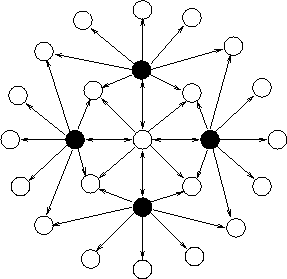
\includegraphics[scale=.5]{mpr.png}
\caption{Flooding a packet in a wireless multi-hop network from the center node using MPRs(black)}
\end{figure}


\subsubsection{Topology Control (TC) Message}
OLSR uses topology control (TC) messages along with MPR forwarding to disseminate neighbor information throughout the network. TC messages are forwarded like usual broadcast messages in the entire network. A TC message is sent periodically by each node in the network to declare its MPR Selector set, i.e., the message contains the list of neighbors who have selected the sender node as a multipoint relay. The sequence number associated to this MPR Selector set is also attached to the list.The information diffused in the network by these TC messages will help each node to build its topology table. A node which has an empty MPR Selector set, i.e., nobody has selected it as a multipoint relay, may not generate any TC message.

\subsubsection{Core Functionality}
Nodes in the network start working by broadcasting HELLO messages to their
neighbors to detect direct one-hop neighbors and also two-hop neighbors. Then,
nodes will try to create and send their TC message in the entire network. These
messages then allow nodes to update their routing tables for different nodes in the
network. To construct the routing table of a node, a shortest path algorithm is used. It means that this routing protocol selects shorter paths by applying Dijkstra’s algorithm. Every routing table consists of destination addresses, next nodes along
the path to the destination, distance from the node to the destination, etc. 

After broadcasting HELLO and TC messages regularly and if the network does
not change, all nodes have the topological information of the entire network, such
as distance from different nodes, one-hop neighbors of every node, next node to the
destination, etc.
\section{Related Works}
Simulation is one of the important tool for assessing the
performance of routing protocols in a Wireless scenario. Till
date, the performance evaluation of most ad hoc routing
protocols has been carried out in a simulation test bed using
NS-2. Recently, a new network simulator called NS-3 which is in its developing stage, demands a great
potential (as claimed by the developers group) for performance analysis of different routing protocols [5].
The performance analysis of AODV in WMNs has been done using ns-3 [6]. OLSR protocol is also a comparatively newer protocol for mobile ad hoc networks [7]. Performance of OLSR protocol is analyzed in [8] and [9]. An improved OLSR protocol which is simulated under ns-3 is also proposed in [10]. 

\chapter{Methodology}

\section{Proposed Methodology}
In our suggested method, when a node sends a
packet to other nodes within its own radio range,
packages will be transmitted by nodes called MPR to
the other nodes. Consequently, if the packet falls into
a loop, then two cases occur; (1) if the package used
less number of steps (less than 255 steps) to reach the
destination, and the packet is IP Header, then we set
dynamically its number of steps to zero to give the
packet the second chance to reach the destination, and
(2) if the package used more number of steps (more
than 255 steps), and the subjected package is not IP
Header, then we eliminate the packet, because,
otherwise, many packets will remain in the network
and this will cause network traffic, bandwidth
occupation, high level of delay in the packet delivery,
and finally, the reduction of package delivery rate and
network payload rate.

\begin{figure}[hbtp]
\centering
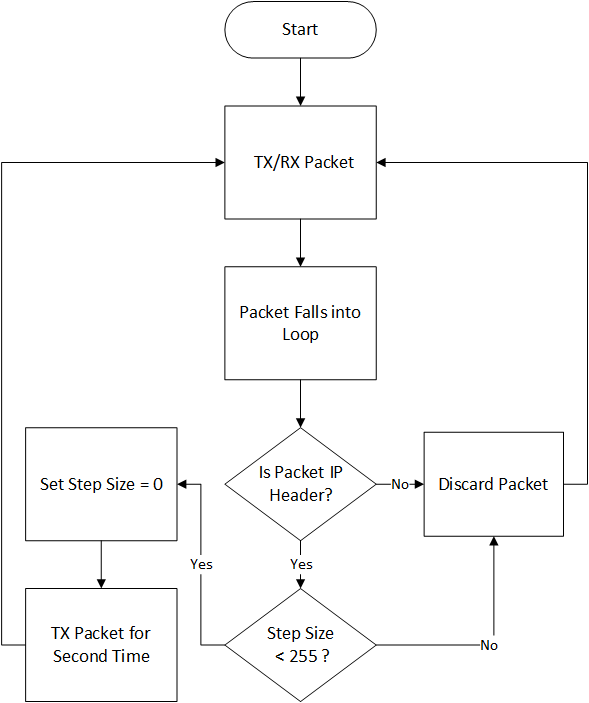
\includegraphics[scale=.6]{Final-Methodology.png}
\caption{Proposed Methodology to Improve OLSR protocol}
\end{figure}


\chapter{Implementation}

\section{Implementation Tools}
The necessary tools to implement this system can be divided in to two categories-Hardware \& Software as described below:
\begin{itemize}
\item 
Hardware Requirements
\begin{itemize}
\item 
Personal Computer with basic configuration
\end{itemize}
\item 
Software Tools
\begin{itemize}
\item 
Operating System: Ubuntu 14.04.1 LTS
\item 
Network Simulator 3 version 3.21
\item 
NetAnim
\item 
PyViz
\item 
Wireshark
\item 
Flow Monitor
\item 
GNU Plot
\end{itemize}
\end{itemize}
\section{Implementation Details}
As discussed in the previous chapter, different routing protocols have been implemented in NS-3 to analyze the performance through experiments. Modification of OLSR has been added to NS-3 source code and it has been recompiled to see the changes. 

\section{Simulation Parameters}
\begin{itemize}
\item 
Number of Nodes: 17, 27, 41
\item 
Simulation Time: 120 seconds
\item 
Mobility Model: RandomWalk2d 
\item 
Routing Protocol: HWMP, AODV, OLSR
\item 
Size of packets: 1024 bytes
\item 
Data Rate of Point to Point links: 100Mbps
\item
Delay in Point to Point links: 10ms
\item 
Data Rate of CSMA connection: 100Mbps
\item
Delay in CSMA connection: 6560ns
\item
Node Distance: 40 meters
\end{itemize}

\section{Simulation Visualization}
The network model used in our simulation is shown in Figure 4.1. The mesh backbone size varies when mesh routers are added in the network. The link between Access Point and Mesh Router is a CSMA link. Mesh Router/Gateway and Internet are connected with Point to Point link. All other connections are wireless.
\begin{figure}[hbtp]
\centering
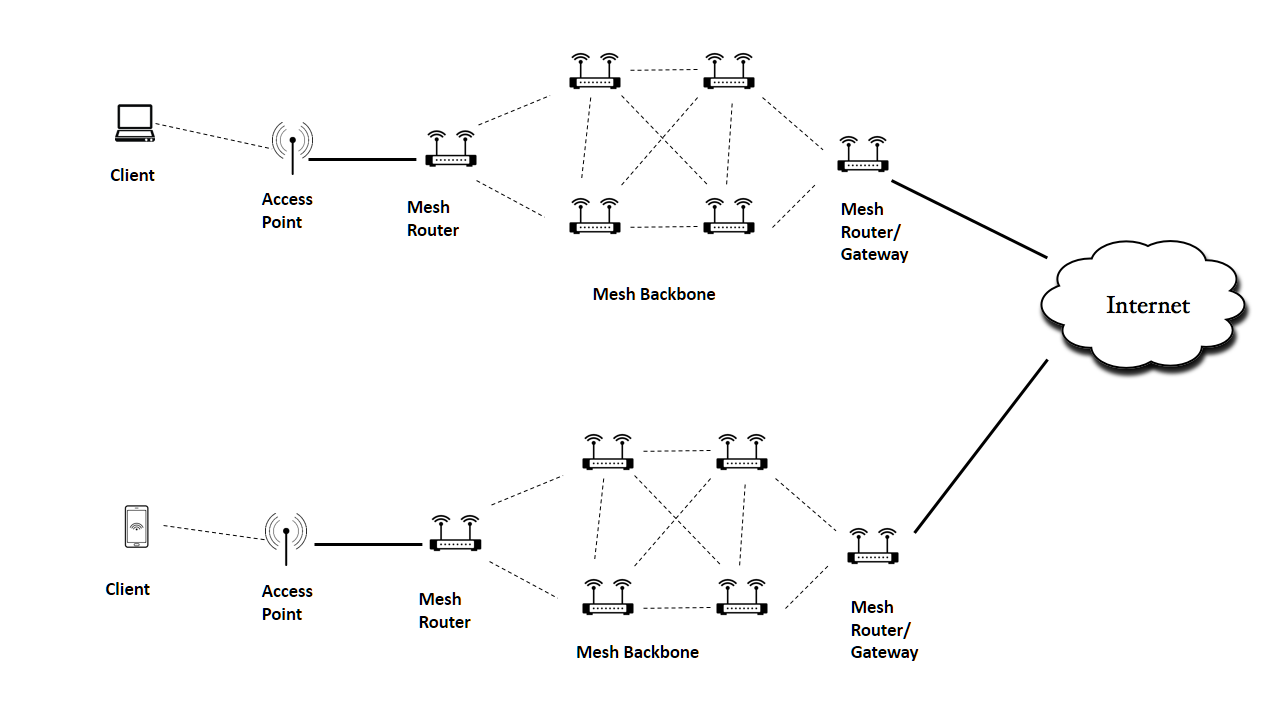
\includegraphics[scale=.5]{Network-Model.png}
\caption{Network Model for Simulation}
\end{figure}
\newpage

The network model shown above is simulated in PyViz as below:
\begin{figure}[hbtp]
\centering
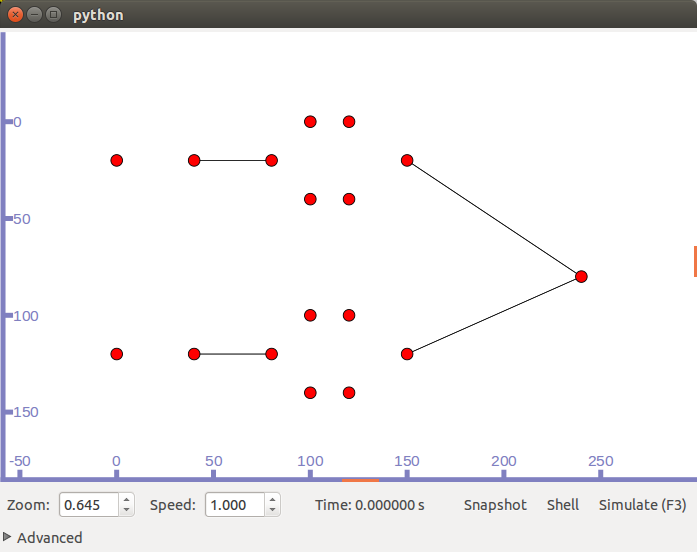
\includegraphics[scale=.4]{mesh-2x2.png}
\caption{Network Model with 4 Mesh Backbone Router}
\end{figure}


\begin{figure}[hbtp]
\centering
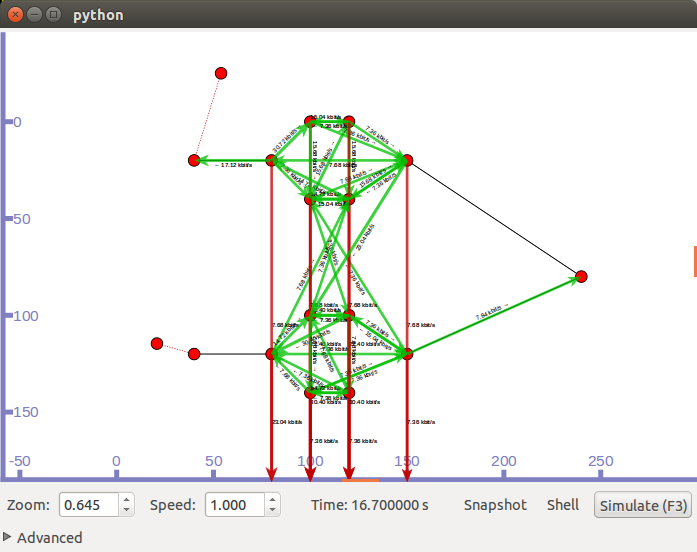
\includegraphics[scale=.45]{mesh-2x2-working.png}
\caption{Data Connectivity across the Network}
\end{figure}


\chapter{Simulation Results and Analysis}

\section{Parameters for Evaluating Simulation Model}
The following parameters are needed for evaluating our simulation:
\begin{itemize}


\item{\textbf{Average Throughput:}}
Number of bits received divided by the difference between the arrival time of the first packet and the last one.
$$Throughput = \frac{Bits\ Received}{timeLastRxPacket - timeFirstTxPacket} $$

\item{\textbf{Average Packet Delivery Fraction (PDF):}}
Number of packets received divided by the number of packets transmitted.
$$PDF = \frac{No.\ of\ Packets\ Received}{No.\ of\ Packets\ Transmitted}$$
\item{\textbf{Average end-to-end Delay:}}
The sum of the delay of all received packets divided by the number of received packets.
$$ETE\ Delay =  \frac{\sum\nolimits Delay\ of\ all\ received\ packets\ }{number\ of\ received\ packets}  $$
\end{itemize}

\newpage
\subsection{Performance Analysis of HWMP, OLSR and AODV Protocol}

\subsubsection{Packet Delivery Fraction (PDF)}

\begin{figure}[hbtp]
\centering
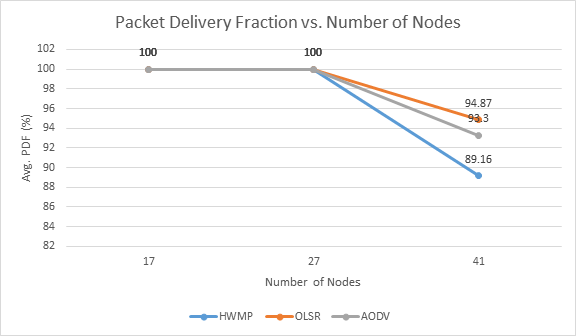
\includegraphics[scale=.7]{Graphs/PDF-vs-nodes.png}
\caption{Performance Analysis in terms of Packet Delivery Fractions}
\end{figure}
In terms of Packet Delivery Fraction, OLSR performs better than HWMP and AODV with the increasing number of nodes. OLSR is particularly suitable for large and dense networks, as the optimization is done using the multipoint relays.

%\newpage

\subsubsection{Throughput}

\begin{figure}[hbtp]
\centering
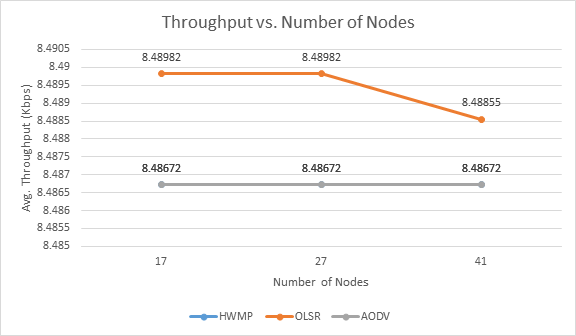
\includegraphics[scale=.7]{Graphs/Throghput-vs-nodes.png}
\caption{Performance Analysis in terms of Throughput}
\end{figure}
As HWMP is based on AODV, the throughput remains the same of these two protocols with the increasing number of nodes. Again, OLSR performs better than the other two routing protocols.
\newpage

\subsubsection{End-to-end Delay}

\begin{figure}[hbtp]
\centering
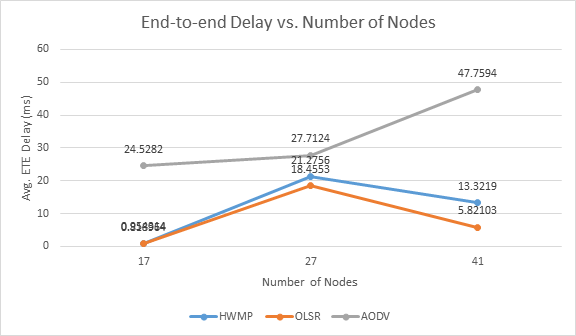
\includegraphics[scale=.7]{Graphs/ETE-vs-nodes.png}
\caption{Performance Analysis in terms of End-to-end Delay}
\end{figure}

In terms of End-to-end delay, OLSR performs better than HWMP and AODV. In OLSR, the optimization is done using the multipoint relays. As the number of nodes increase, number of MPRs also increases. These increased MPRs can optimize the network performance.


\subsection{Performance Analysis of OLSR and Improved OLSR}
\subsubsection{Packet Delivery Fraction}
\begin{figure}[hbtp]
\centering
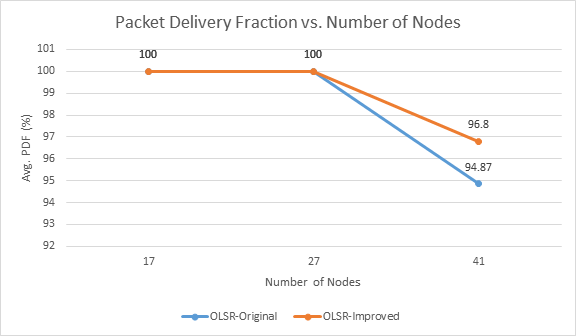
\includegraphics[scale=.7]{Graphs/OLSR-pdf-vs-nodes.png}
\caption{Comparison of PDF between Original OLSR and Improved OLSR}
\end{figure}

In terms of Packet Delivery Ratio, our improved OLSR performs well when the node number increases. As more number of packets get the chance to reach the destination, PDF also increases. 

\newpage

\subsubsection{Throughput}

\begin{figure}[hbtp]
\centering
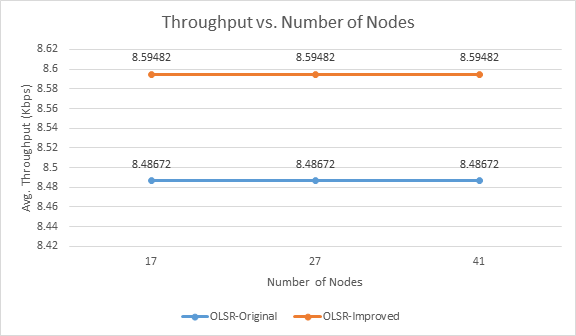
\includegraphics[scale=.7]{Graphs/OLSR-throughput-vs-nodes.png}
\caption{Comparison of Throughput between Original OLSR and Improved OLSR}
\end{figure}

In terms of Throughput, our improved OLSR performs better than the original one. The number of packets that reach the destination is higher in our method. So, the throughput also increases.



\subsubsection{End-to-end Delay}

\begin{figure}[hbtp]
\centering
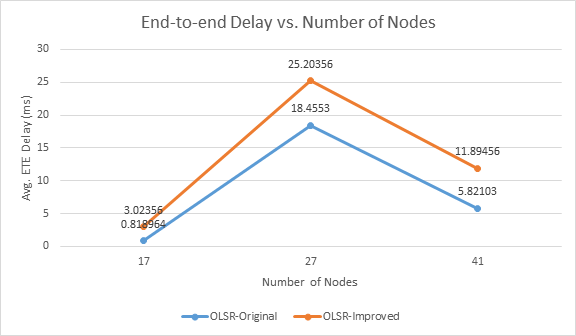
\includegraphics[scale=.7]{Graphs/OLSR-ete-vs-nodes.png}
\caption{Comparison of End-to-end Delay between Original OLSR and Improved OLSR}
\end{figure}

In terms of End-to-end delay, original OLSR performs better than our proposed method. As the packets get second chance to reach to the destination, the end-to-end delay increases in our method. 


\newpage
\section{Overall Performance Analysis}
% Please add the following required packages to your document preamble:
% \usepackage{multirow}
\begin{table}[h]
\begin{tabular}{|c|c|c|c|c|}
\hline
\multicolumn{1}{|l|}{Protocol} & No. of Nodes & Avg. Throughput (Kbps) & Avg. ETE Delay (ms) & \multicolumn{1}{l|}{Avg. PDF (\%)} \\ \hline
\multirow{3}{*}{HWMP} & 17 & 8.48672 & 0.954314 & 100 \\ \cline{2-5} 
 & 27 & 8.48672 & 21.2756 & 100 \\ \cline{2-5} 
 & 41 & 8.48672 & 13.3219 & 89.16 \\ \hline
\multirow{3}{*}{OLSR} & 17 & 8.48982 & 0.818964 & 100 \\ \cline{2-5} 
 & 27 & 8.48855 & 18.4553 & 100 \\ \cline{2-5} 
 & 41 & 8.48855 & 5.82103 & 94.87 \\ \hline
\multirow{3}{*}{AODV} & 17 & 8.48672 & 24.5282 & 100 \\ \cline{2-5} 
 & 27 & 8.48672 & 27.7124 & 100 \\ \cline{2-5} 
 & 41 & 8.48672 & 47.7594 & 93.3 \\ \hline
\multirow{3}{*}{\begin{tabular}[c]{@{}c@{}}Improved\\ OLSR\end{tabular}} & 17 & 8.59482 & 3.02356 & 100 \\ \cline{2-5} 
 & 27 & 8.59482 & 25.20356 & 100 \\ \cline{2-5} 
 & 41 & 8.59482 & 18.4553 & 96.8 \\ \hline
\end{tabular}
\caption{Overall Performance Analysis}
\label{Overall Performance Analysis}

\end{table}

From the above information, it is clearly shown that OLSR protocol performs better than HWMP and AODV with different network size. However, our improved OLSR protocol is definitely performs better than original OLSR in terms of Packet Delivery Ratio and Throughput.

\chapter{Conclusion}
\section{Findings of the Work}
In this research we focused on the performance of HWMP, AODV and OLSR protocols. The
implementation of the simulation has been done in NS-3 and with the results we have evaluated
the performance of  HWMP, AODV and OLSR protocol. In most of the cases we have seen that the
performance of OLSR is slightly better than HWMP and AODV. We also improved the OLSR routing
protocol by eliminating the unnecessary loops. The
results of the simulation show that the changed OLSR
routing protocol (the suggested method) causes a
significant improvement in the criteria of Packet Delivery Fraction and Throughput.
\section{Future Improvements}

We will use OLSR protocol on more complex and complicated scenario. We are also planning
to implement our project with more different parameters. In future we will compare OLSR with
some other better protocols. OLSR could be an important field to research which would help to
improve its performance on a specified wireless mesh network.

%\nocite{*}

%\bibliographystyle{plain}
%\bibliography{thesis}

%\printbibliography

\appendices
\chapter{Source Code}

%\inputminted{cpp}{infrastructure-mesh-backbone.cc}

\begin{verbatim}
/* -*-  Mode: C++; c-file-style: "gnu"; indent-tabs-mode:nil; -*- */
/*
 *
 *
 * Author: Fahim Masud Choudhury <fahim.cuet@gmail.com>
 *         Hasanuzzaman Noor     <zaman.cuet@gmail.com>
 *         Md. Monowar Hossain   <murad0904045@gmail.com>
 */

#include "ns3/core-module.h"
#include "ns3/internet-module.h"
#include "ns3/network-module.h"
#include "ns3/applications-module.h"
#include "ns3/wifi-module.h"
#include "ns3/mesh-module.h"
#include "ns3/mobility-module.h"
#include "ns3/mesh-helper.h"
#include "ns3/flow-monitor-module.h"
#include <iomanip>
#include <string>
#include <iostream>
#include <sstream>
#include <fstream>
#include <ns3/flow-monitor-helper.h>
#include "ns3/gnuplot.h"
#include "ns3/netanim-module.h"
#include "src/point-to-point/helper/point-to-point-helper.h"
#include "src/csma/helper/csma-helper.h"
#include "ns3/olsr-helper.h"
#include "ns3/ipv4-global-routing-helper.h"
#include "ns3/netanim-module.h"
#include "src/network/model/packet-metadata.h"
//#include "mesh.h"

#include <iostream>
#include <sstream>
#include <fstream>
using namespace ns3;

NS_LOG_COMPONENT_DEFINE ("infrastructure-mesh");
void ThroughputMonitor (FlowMonitorHelper *fmhelper, Ptr<FlowMonitor> flowMon, Gnuplot2dDataset DataSet);
// Method for setting mobility using (x,y) position for the nodes

static void
SetPosition (Ptr<Node> node, double x, double y)
{
  Ptr<MobilityModel> mobility = node->GetObject<MobilityModel> ();
  Vector pos = mobility->GetPosition ();
  pos.x = x;
  pos.y = y;
  mobility->SetPosition (pos);
}

class MeshTest
{
public:
  /// Init test
  MeshTest ();
  /// Configure test from command line arguments
  void Configure (int argc, char ** argv);
  /// Run test
  int Run ();
private:
  int m_xSize;
  int m_ySize;
  int m_backbone;
  int m_gw;
  //int m_mr;
  int m_ap;
  int m_sta;
  double m_step;
  double m_randomStart;
  double m_totalTime;
  double m_packetInterval;
  uint16_t m_packetSize;
  uint32_t m_nIfaces;
  bool m_chan;
  bool m_pcap;
  std::string m_stack;
  std::string m_phyMode;
  std::string m_rate;
  std::string m_root;

  /// NodeContainer for individual nodes
  NodeContainer nc_sta1, nc_sta2;
  NodeContainer nc_ap1, nc_ap2;
  NodeContainer nc_mr1, nc_mr2;
  NodeContainer nc_mbb1, nc_mbb2;
  NodeContainer nc_gw1, nc_gw2;
  NodeContainer nc_bb1;

  // NodeContainer for categorical nodes
  NodeContainer nc_sta, nc_ap, nc_mesh1, nc_mesh2;

  // NodeContainer for connected nodes
  NodeContainer nc_sta1Ap1, nc_sta2Ap2;
  NodeContainer nc_ap1Mr1, nc_ap2Mr2;
  NodeContainer nc_mr1Mbb1, nc_mr2Mbb2;
  NodeContainer nc_mbb1Gw1, nc_mbb2Gw2;
  NodeContainer nc_gw1Bb1, nc_gw2Bb1;


  // List of categorical NetDevice Container
  NetDeviceContainer de_sta1, de_sta2;
  NetDeviceContainer de_ap1, de_ap2;

  // List of WiFi NetDevice Container
  NetDeviceContainer de_wifi_sta1Ap1;
  NetDeviceContainer de_wifi_sta2Ap2;

  // List of mesh NetDevice Container
  NetDeviceContainer de_mesh1;
  NetDeviceContainer de_mesh2;

  NetDeviceContainer de_mesh_mbb1Gw1;
  NetDeviceContainer de_mesh_mbb2Gw2;

  NetDeviceContainer de_mesh_mr1Mbb1;
  NetDeviceContainer de_mesh_mr2Mbb2;

  // List of CSMA NetDevice Container
  NetDeviceContainer de_csma_ap1Mr1;
  NetDeviceContainer de_csma_ap2Mr2;

  // List of p2p NetDevice Container
  NetDeviceContainer de_p2p_gw1Bb1;
  NetDeviceContainer de_p2p_gw2Bb1;

  // List of interface container
  Ipv4InterfaceContainer if_wifi_sta1Ap1;
  Ipv4InterfaceContainer if_wifi_sta2Ap2;

  Ipv4InterfaceContainer if_mesh_mr1Mbb1;
  Ipv4InterfaceContainer if_mesh_mr2Mbb2;

  Ipv4InterfaceContainer if_mesh1;
  Ipv4InterfaceContainer if_mesh2;

  Ipv4InterfaceContainer if_csma_ap1Mr1;
  Ipv4InterfaceContainer if_csma_ap2Mr2;

  Ipv4InterfaceContainer if_p2p_gw1Bb1;
  Ipv4InterfaceContainer if_p2p_gw2Bb1;

  // Helper
  MeshHelper meshHelper1, meshHelper2;
  PointToPointHelper p2pHelper;
  CsmaHelper csmaHelper;
  Ipv4AddressHelper address;

private:
  /// Create nodes and setup their mobility
  void CreateNodes ();
  /// Install internet m_stack on nodes
  void InstallInternetStack ();
  /// Setup mobility
  void SetupMobility ();
  /// Install applications
  void InstallApplication ();
  /// Print mesh devices diagnostics
  void Report ();
};

MeshTest::MeshTest () :
m_xSize (3),
m_ySize (3),
m_backbone (1),
//m_mesh (6),
m_gw (2),
m_ap (2),
m_sta (2),
m_step (40.0),
m_randomStart (0.1),
m_totalTime (50.0),
m_packetInterval (1.0),
m_packetSize (1024),
m_nIfaces (1),
m_chan (true),
m_pcap (false),
m_stack ("ns3::Dot11sStack"),
m_phyMode ("DsssRate1Mbps"),
m_rate ("8kbps"),
m_root ("ff:ff:ff:ff:ff:ff") { }

void
MeshTest::Configure (int argc, char *argv[])
{
  CommandLine cmd;
  cmd.AddValue ("phymode", "Wifi Phy mode", m_phyMode);
  cmd.AddValue ("x-size", "Number of nodes in a row grid. [6]", m_xSize);
  cmd.AddValue ("y-size", "Number of rows in a grid. [6]", m_ySize);
  cmd.AddValue ("step", "Size of edge in our grid, meters. [100 m]", m_step);
  /*
   * As soon as starting node means that it sends a beacon,
   * simultaneous start is not good.
   */
  cmd.AddValue ("start", "Maximum random start delay, seconds. [0.1 s]", m_randomStart);
  cmd.AddValue ("time", "Simulation time, seconds [100 s]", m_totalTime);
  cmd.AddValue ("packet-interval", "Interval between packets in UDP ping, seconds [0.001 s]", m_packetInterval);
  cmd.AddValue ("packet-size", "Size of packets in UDP ping", m_packetSize);
  cmd.AddValue ("interfaces", "Number of radio interfaces used by each mesh point. [1]", m_nIfaces);
  cmd.AddValue ("channels", "Use different frequency channels for different interfaces. [0]", m_chan);
  cmd.AddValue ("pcap", "Enable PCAP traces on interfaces. [0]", m_pcap);
  cmd.AddValue ("stack", "Type of protocol stack. ns3::Dot11sStack by default", m_stack);
  cmd.AddValue ("root", "Mac address of root mesh point in HWMP", m_root);

  cmd.Parse (argc, argv);
  //NS_LOG_DEBUG("Grid:" << m_xSize << "*" << m_ySize);
  //NS_LOG_DEBUG("Simulation time: " << m_totalTime << " s");
  Config::SetDefault ("ns3::OnOffApplication::DataRate",
                      StringValue (m_rate));

}

void
MeshTest::CreateNodes ()
{
  // Create individual nodes in their node container
  nc_sta1.Create (1);
  nc_sta2.Create (1);
  nc_ap1.Create (1);
  nc_ap2.Create (1);
  nc_mr1.Create (1);
  nc_mr2.Create (1);
  nc_mbb1.Create (m_ySize * m_xSize);
  nc_mbb2.Create (m_ySize * m_xSize);
  nc_gw1.Create (1);
  nc_gw2.Create (1);
  nc_bb1.Create (1);

  // Create categorical Node Container
  nc_sta = NodeContainer (nc_sta1, nc_sta2);
  nc_ap = NodeContainer (nc_ap1, nc_ap2);

  // Create connected nodes in their node container
  nc_sta1Ap1 = NodeContainer (nc_sta1, nc_ap1);
  nc_sta2Ap2 = NodeContainer (nc_sta2, nc_ap2);
  nc_ap1Mr1 = NodeContainer (nc_ap1, nc_mr1);
  nc_ap2Mr2 = NodeContainer (nc_ap2, nc_mr2);
  nc_mr1Mbb1 = NodeContainer (nc_mr1, nc_mbb1);
  nc_mr2Mbb2 = NodeContainer (nc_mr2, nc_mbb2);
  nc_mbb1Gw1 = NodeContainer (nc_mbb1, nc_gw1);
  nc_mbb2Gw2 = NodeContainer (nc_mbb2, nc_gw2);
  nc_gw1Bb1 = NodeContainer (nc_gw1, nc_bb1);
  nc_gw2Bb1 = NodeContainer (nc_gw2, nc_bb1);

  nc_mesh1 = NodeContainer (nc_mr1, nc_mbb1, nc_gw1);
  nc_mesh2 = NodeContainer (nc_mr2, nc_mbb2, nc_gw2);

  // Create p2p links between backbone (bb1) and gateways (gw1, gw2)
  p2pHelper.SetDeviceAttribute ("DataRate", StringValue ("100Mbps"));
  p2pHelper.SetChannelAttribute ("Delay", StringValue ("10ms"));
  de_p2p_gw1Bb1 = p2pHelper.Install (nc_gw1Bb1);
  de_p2p_gw2Bb1 = p2pHelper.Install (nc_gw2Bb1);

  // Create CSMA connection between MRs (mr1, mr2) and APs (ap1, ap2)
  csmaHelper.SetChannelAttribute ("DataRate", StringValue ("100Mbps"));
  csmaHelper.SetChannelAttribute ("Delay", TimeValue (NanoSeconds (6560)));
  de_csma_ap1Mr1 = csmaHelper.Install (nc_ap1Mr1);
  de_csma_ap2Mr2 = csmaHelper.Install (nc_ap2Mr2);

  // Configure YansWifiChannel
  YansWifiPhyHelper wifiPhy = YansWifiPhyHelper::Default ();
  YansWifiChannelHelper wifiChannel = YansWifiChannelHelper::Default ();
  wifiPhy.SetChannel (wifiChannel.Create ());

  //------------------------ mesh router1 -----------------------------------
  /*
   * Create mesh helper and set stack installer to it
   * Stack installer creates all needed protocols and install them to
   * mesh point device
   */
  meshHelper1 = MeshHelper::Default ();
  if (!Mac48Address (m_root.c_str ()).IsBroadcast ())
    {
      meshHelper1.SetStackInstaller (m_stack, "Root", Mac48AddressValue (Mac48Address (m_root.c_str ())));
    }
  else
    {
      //If root is not set, we do not use "Root" attribute, because it
      //is specified only for 11s
      meshHelper1.SetStackInstaller (m_stack);
    }
  if (m_chan)
    {
      meshHelper1.SetSpreadInterfaceChannels (MeshHelper::SPREAD_CHANNELS);
    }
  else
    {
      meshHelper1.SetSpreadInterfaceChannels (MeshHelper::ZERO_CHANNEL);
    }
  meshHelper1.SetMacType ("RandomStart", TimeValue (Seconds (m_randomStart)));
  // Set number of interfaces - default is single-interface mesh point
  meshHelper1.SetNumberOfInterfaces (m_nIfaces);
  // Install protocols and return container if MeshPointDevices
  de_mesh1 = meshHelper1.Install (wifiPhy, nc_mesh1);

  //----------------------mesh router2 ------------------------------------------

  meshHelper2 = MeshHelper::Default ();
  if (!Mac48Address (m_root.c_str ()).IsBroadcast ())
    {
      meshHelper2.SetStackInstaller (m_stack, "Root", Mac48AddressValue (Mac48Address (m_root.c_str ())));
    }
  else
    {
      //If root is not set, we do not use "Root" attribute, because it
      //is specified only for 11s
      meshHelper2.SetStackInstaller (m_stack);
    }
  if (m_chan)
    {
      meshHelper2.SetSpreadInterfaceChannels (MeshHelper::SPREAD_CHANNELS);
    }
  else
    {
      meshHelper2.SetSpreadInterfaceChannels (MeshHelper::ZERO_CHANNEL);
    }
  meshHelper2.SetMacType ("RandomStart", TimeValue (Seconds (m_randomStart)));
  // Set number of interfaces - default is single-interface mesh point
  meshHelper2.SetNumberOfInterfaces (m_nIfaces);

  de_mesh2 = meshHelper2.Install (wifiPhy, nc_mesh2);


  // TODO: Setup Mobility for mesh nodes

  // Setup WiFi for network 1
  WifiHelper wifi1 = WifiHelper::Default ();
  wifi1.SetStandard (WIFI_PHY_STANDARD_80211b);
  wifi1.SetRemoteStationManager ("ns3::AarfWifiManager");

  NqosWifiMacHelper mac1 = NqosWifiMacHelper::Default ();
  wifi1.SetRemoteStationManager ("ns3::ConstantRateWifiManager",
                                 "DataMode", StringValue (m_phyMode),
                                 "ControlMode", StringValue (m_phyMode));

  // TODO: Change SSID for different networks
  // Install on different ap1 <--> sta1, ap2 <--> sta2

  // STA1 and AP1 are initialized for network 1
  Ssid ssid1 = Ssid ("network-1");
  mac1.SetType ("ns3::StaWifiMac",
                "Ssid", SsidValue (ssid1),
                "ActiveProbing", BooleanValue (true));

  de_sta1 = wifi1.Install (wifiPhy, mac1, nc_sta1);

  // Setup AP for network 1
  mac1.SetType ("ns3::ApWifiMac",
                "Ssid", SsidValue (ssid1));

  de_ap1 = wifi1.Install (wifiPhy, mac1, nc_ap1);

  // Setup WiFi for network 2
  WifiHelper wifi2 = WifiHelper::Default ();
  wifi2.SetStandard (WIFI_PHY_STANDARD_80211b);
  wifi2.SetRemoteStationManager ("ns3::AarfWifiManager");

  NqosWifiMacHelper mac2 = NqosWifiMacHelper::Default ();
  wifi2.SetRemoteStationManager ("ns3::ConstantRateWifiManager",
                                 "DataMode", StringValue (m_phyMode),
                                 "ControlMode", StringValue (m_phyMode));

  // STA and APs are initialized for network 2
  Ssid ssid2 = Ssid ("network-2");
  mac2.SetType ("ns3::StaWifiMac",
                "Ssid", SsidValue (ssid2),
                "ActiveProbing", BooleanValue (true));

  de_sta2 = wifi2.Install (wifiPhy, mac2, nc_sta2);

  // Setup AP for network 2
  mac2.SetType ("ns3::ApWifiMac",
                "Ssid", SsidValue (ssid2));

  de_ap2 = wifi2.Install (wifiPhy, mac2, nc_ap2);

  // Net Device container for STA and AP in network 1
  de_wifi_sta1Ap1.Add (de_sta1);
  de_wifi_sta1Ap1.Add (de_ap1);

  // Net Device container for STA and AP in network 2
  de_wifi_sta2Ap2.Add (de_sta2);
  de_wifi_sta2Ap2.Add (de_ap2);

}

void
MeshTest::SetupMobility ()
{
  // Setup mobility for the nodes
  MobilityHelper fixedMobility;
  fixedMobility.SetPositionAllocator ("ns3::GridPositionAllocator",
                                      "MinX", DoubleValue (0.0),
                                      "MinY", DoubleValue (((m_xSize - 1) * m_step) / 2),
                                      "DeltaX", DoubleValue (m_step),
                                      "DeltaY", DoubleValue (m_step),
                                      "GridWidth", UintegerValue (5),
                                      "LayoutType", StringValue ("RowFirst"));

  fixedMobility.SetMobilityModel ("ns3::RandomWalk2dMobilityModel",
                                  "Bounds", RectangleValue (Rectangle (-75, 75, -75, 75)),
                                  "Speed", StringValue ("ns3::UniformRandomVariable[Min=20.0|Max=50.0]"),
                                  "Direction",StringValue ("ns3::UniformRandomVariable[Min=10.0|Max=26.283184]"));
  fixedMobility.Install (nc_sta1);

  fixedMobility.SetMobilityModel ("ns3::ConstantPositionMobilityModel");


  //fixedMobility.Install(nc_sta1);
  fixedMobility.Install (nc_ap1);
  fixedMobility.Install (nc_mr1);
  fixedMobility.Install (nc_gw1);
  fixedMobility.Install (nc_bb1);



  // -------------------------------Setup mobility for the nodes---------------------
  MobilityHelper fixedMobility2;
  fixedMobility2.SetPositionAllocator ("ns3::GridPositionAllocator",
                                       "MinX", DoubleValue ((3 * m_step)-(m_step / 2)),
                                       "MinY", DoubleValue (0.0),
                                       "DeltaX", DoubleValue (m_step / 2),
                                       "DeltaY", DoubleValue (m_step),
                                       "GridWidth", UintegerValue (m_xSize),
                                       "LayoutType", StringValue ("RowFirst"));
  fixedMobility2.SetMobilityModel ("ns3::ConstantPositionMobilityModel");


  // ------------------------Setup fixed position for the network nodes----------------

  fixedMobility2.Install (nc_mbb1);



  MobilityHelper fixedMobility3;
  fixedMobility3.SetPositionAllocator ("ns3::GridPositionAllocator",
                                       "MinX", DoubleValue (0.0),
                                       "MinY", DoubleValue ((((m_xSize - 1) * m_step) + m_step)+(((m_xSize - 1) * m_step))),
                                       "DeltaX", DoubleValue (m_step),
                                       "DeltaY", DoubleValue (m_step),
                                       "GridWidth", UintegerValue (5),
                                       "LayoutType", StringValue ("RowFirst"));

  fixedMobility3.SetMobilityModel ("ns3::RandomWalk2dMobilityModel",
                                   "Bounds", RectangleValue (Rectangle (-250, 250, -250, 250)),
                                   "Speed", StringValue ("ns3::UniformRandomVariable[Min=10.0|Max=25.0]"),
                                   "Direction",StringValue ("ns3::UniformRandomVariable[Min=10.0|Max=26.283184]"));
  
  fixedMobility3.Install (nc_sta2);

  fixedMobility3.SetMobilityModel ("ns3::ConstantPositionMobilityModel");

  // Setup fixed position for the network nodes

  //fixedMobility3.Install(nc_sta2);
  fixedMobility3.Install (nc_ap2);
  fixedMobility3.Install (nc_mr2);
  fixedMobility3.Install (nc_gw2);


  MobilityHelper fixedMobility4;
  fixedMobility4.SetPositionAllocator ("ns3::GridPositionAllocator",
                                       "MinX", DoubleValue ((3 * m_step)-(m_step / 2)),
                                       "MinY", DoubleValue (((((m_xSize - 1) * m_step) / 2)*3) + m_step),
                                       "DeltaX", DoubleValue (m_step / 2),
                                       "DeltaY", DoubleValue (m_step),
                                       "GridWidth", UintegerValue (m_xSize),
                                       "LayoutType", StringValue ("RowFirst"));
  fixedMobility4.SetMobilityModel ("ns3::ConstantPositionMobilityModel");

  fixedMobility4.Install (nc_mbb2);


  // possition for bb1, gw1, gw2
  int m_x = ((2 + m_xSize) * m_step) +(2 * m_step);
  int m_y = ((m_xSize * 2) * m_step) / 2;



  SetPosition (nc_bb1.Get (0), m_x, m_y);
  SetPosition (nc_gw1.Get (0), ((m_xSize + 2) * m_step) - m_step, (((m_xSize - 1) * m_step) / 2));
  SetPosition (nc_gw2.Get (0), ((m_xSize + 2) * m_step) - m_step, ((((m_xSize - 1) * m_step) + m_step)+(((m_xSize - 1) * m_step))));

//  SetPosition(nc_gw1.Get(0), 150, 20);
//  SetPosition(nc_gw2.Get(0), 150, 120);
  
  // Setup mobility for the STA1 node
  double startTime = 20.0;

  for (int sta1_x = 0, sta1_y = 0; sta1_y >= -15; sta1_x++, sta1_y -= 3)
    {
      // Change position of STA1 after startTime
      Simulator::Schedule (Seconds (startTime), &SetPosition, nc_sta1.Get (0), sta1_x, sta1_y);

      startTime++;
    }

  // Position STA1 node from AP1 network to AP2 network
  //Simulator::Schedule (Seconds (20.0), &SetPosition, nc_sta1.Get (0), 10.0, 15.0);
  // Position STA2 node from AP2 network to AP2 network
  //Simulator::Schedule (Seconds (20.0), &SetPosition, nc_sta2.Get (0), 0.0, 0.0);


}

void
MeshTest::InstallInternetStack ()
{

  InternetStackHelper internetStackHelper;
  OlsrHelper routingProtocol;
  internetStackHelper.SetRoutingHelper (routingProtocol);

  // Setup internet stack on the nodes
  internetStackHelper.Install (nc_sta1);
  internetStackHelper.Install (nc_sta2);
  internetStackHelper.Install (nc_ap1);
  internetStackHelper.Install (nc_ap2);
  internetStackHelper.Install (nc_mr1);
  internetStackHelper.Install (nc_mr2);
  internetStackHelper.Install (nc_mbb1);
  internetStackHelper.Install (nc_mbb2);
  internetStackHelper.Install (nc_gw1);
  internetStackHelper.Install (nc_gw2);
  internetStackHelper.Install (nc_bb1);

  // Network 1 (left)
  address.SetBase ("10.1.1.0", "255.255.255.0");
  if_wifi_sta1Ap1 = address.Assign (de_wifi_sta1Ap1);

  address.SetBase ("10.1.2.0", "255.255.255.0");
  if_csma_ap1Mr1 = address.Assign (de_csma_ap1Mr1);

  address.SetBase ("10.1.3.0", "255.255.255.0");
  if_mesh1 = address.Assign (de_mesh1);

  address.SetBase ("10.1.4.0", "255.255.255.0");
  if_p2p_gw1Bb1 = address.Assign (de_p2p_gw1Bb1);

  // Network 2 (right)
  address.SetBase ("20.1.1.0", "255.255.255.0");
  if_wifi_sta2Ap2 = address.Assign (de_wifi_sta2Ap2);

  address.SetBase ("20.1.2.0", "255.255.255.0");
  if_csma_ap2Mr2 = address.Assign (de_csma_ap2Mr2);

  address.SetBase ("20.1.3.0", "255.255.255.0");
  if_mesh2 = address.Assign (de_mesh2);

  address.SetBase ("20.1.4.0", "255.255.255.0");
  if_p2p_gw2Bb1 = address.Assign (de_p2p_gw2Bb1);

}

void
MeshTest::InstallApplication ()
{
  // Server is set on STA2 in network 2 (right)
  UdpEchoServerHelper echoServer (9);
  ApplicationContainer serverApps = echoServer.Install (nc_sta2.Get (0));
  serverApps.Start (Seconds (0.0));
  serverApps.Stop (Seconds (m_totalTime));

  // Client is set on STA1 in network 1 (left)
  UdpEchoClientHelper echoClient (if_wifi_sta2Ap2.GetAddress (0), 9);
  echoClient.SetAttribute ("MaxPackets", UintegerValue ((uint32_t) (m_totalTime * (1 / m_packetInterval))));
  echoClient.SetAttribute ("Interval", TimeValue (Seconds (m_packetInterval)));
  echoClient.SetAttribute ("PacketSize", UintegerValue (m_packetSize));
  ApplicationContainer clientApps = echoClient.Install (nc_sta1.Get (0));
  clientApps.Start (Seconds (0.0));
  clientApps.Stop (Seconds (m_totalTime));

  //Ipv4GlobalRoutingHelper::PopulateRoutingTables ();
}

int
MeshTest::Run ()
{

  CreateNodes ();
  InstallInternetStack ();
  SetupMobility ();
  InstallApplication ();

  //Gnuplot parameters

  std::string fileNameWithNoExtension = "FlowVSThroughput_ft_";
  std::string graphicsFileName = fileNameWithNoExtension + ".png";
  std::string plotFileName = fileNameWithNoExtension + ".plt";
  std::string plotTitle = "Flow vs Throughput";
  std::string dataTitle = "Throughput";

  // Instantiate the plot and set its title.
  Gnuplot gnuplot (graphicsFileName);
  gnuplot.SetTitle (plotTitle);

  // Make the graphics file, which the plot file will be when it
  // is used with Gnuplot, be a PNG file.
  gnuplot.SetTerminal ("png");

  // Set the labels for each axis.
  gnuplot.SetLegend ("Flow", "Throughput");


  Gnuplot2dDataset dataset;
  dataset.SetTitle (dataTitle);
  dataset.SetStyle (Gnuplot2dDataset::LINES_POINTS);

  //flowMonitor declaration
  FlowMonitorHelper fmHelper;
  Ptr<FlowMonitor> allMon = fmHelper.InstallAll ();
  // call the flow monitor function
  ThroughputMonitor (&fmHelper, allMon, dataset);


  Simulator::Stop (Seconds (m_totalTime));
  // Enable graphical interface for netanim
  AnimationInterface animation ("infrastructure-mesh-backbone.xml");
  animation.EnablePacketMetadata (false);

  Simulator::Run ();
  //Gnuplot ...continued
  gnuplot.AddDataset (dataset);
  // Open the plot file.
  std::ofstream plotFile (plotFileName.c_str ());
  // Write the plot file.
  gnuplot.GenerateOutput (plotFile);
  // Close the plot file.
  plotFile.close ();
  Simulator::Destroy ();

  return 0;
}

int
main (int argc, char *argv[])
{
  ns3::PacketMetadata::Enable ();
  LogComponentEnable ("UdpEchoClientApplication", LOG_LEVEL_INFO);
  LogComponentEnable ("UdpEchoServerApplication", LOG_LEVEL_INFO);
  MeshTest t;
  t.Configure (argc, argv);
  return t.Run ();
}

void
ThroughputMonitor (FlowMonitorHelper *fmhelper, Ptr<FlowMonitor> flowMon, Gnuplot2dDataset DataSet)
{
  double localThrou = 0;
  std::map<FlowId, FlowMonitor::FlowStats> flowStats = flowMon->GetFlowStats ();
  Ptr<Ipv4FlowClassifier> classing = DynamicCast<Ipv4FlowClassifier> (fmhelper->GetClassifier ());
  for (std::map<FlowId, FlowMonitor::FlowStats>::const_iterator stats = flowStats.begin (); stats != flowStats.end (); ++stats)
    {
      Ipv4FlowClassifier::FiveTuple fiveTuple = classing->FindFlow (stats->first);
      std::cout << "Flow ID     : " << stats->first << " ; " << fiveTuple.sourceAddress << " -----> " << fiveTuple.destinationAddress << std::endl;
      std::cout << "Tx Packets = " << stats->second.txPackets << std::endl;
      std::cout << "Rx Packets = " << stats->second.rxPackets << std::endl;
      std::cout << "Duration    : " << (stats->second.timeLastRxPacket.GetSeconds () - stats->second.timeFirstTxPacket.GetSeconds ()) << std::endl;
      std::cout << "Last Received Packet  : " << stats->second.timeLastRxPacket.GetSeconds () << " Seconds" << std::endl;
      std::cout << "Throughput: " << stats->second.rxBytes * 8.0 / (stats->second.timeLastRxPacket.GetSeconds () - stats->second.timeFirstTxPacket.GetSeconds ()) / 1024 / 1024 << " Mbps" << std::endl;
      localThrou = (stats->second.rxBytes * 8.0 / (stats->second.timeLastRxPacket.GetSeconds () - stats->second.timeFirstTxPacket.GetSeconds ()) / 1024 / 1024);
      // updata gnuplot data
      DataSet.Add ((double) Simulator::Now ().GetSeconds (), (double) localThrou);
      std::cout << "---------------------------------------------------------------------------" << std::endl;
    }
  Simulator::Schedule (Seconds (1), &ThroughputMonitor, fmhelper, flowMon, DataSet);
  //if(flowToXml)
  {
    flowMon->SerializeToXmlFile ("infrastructure-mesh-backbone-throughputMonitor.xml", true, true);
  }

}


\end{verbatim}

\end{document}



